\Chapter{Szimulációs környezet}

A szimulációs környezetet a NumPy \cite{harris2020array} nevű Python \cite{python} könyvtár segítségével készítettem el.
Azért előnyös saját környezetet létrehozni, mert így csak azokat a részeket kell tárolni, számolni amelyek számunkra szükségesek.

Ebben a fejezetben a használt osztályok felépítése valamint a szimuláció működése kerül részletezésre.

\Section{A test reprezentációja}

Az adatok tárolásáért és a szimulációs számításokért egyetlen osztály, a \texttt{Dice} felel.
A következőkben bemutatott metódusok ehhez az osztályhoz tartoznak.

\begin{python}
class Dice:
    def __init__(self):
        self.n
        self.partciles = []
        self.springs = []
        self.faces = []
        self.initVerticies()
        self.initSprings()

    def initVertices(self):
        raise NotImplementedError

    def initSprings(self):
        for i in range(self.n - 1):
            for j in range(i + 1, self.n):
                self.springs.append(Spring(self.particles[i],
                                           self.particles[j]))
\end{python}

Az objektumokat egyszerűbb számítások miatt nem szilárdnak tekintjük, hanem pontokból és rugókból álló halmaznak.
Ezért a test felépítéséhez a csúcspontokat , a közéjük kifeszített rugókat, valamint az oldallapokat határoló csúcsok listáját fogjuk eltárolni.
Minden testhez külön kell létrehoznunk egy gyerekosztályt, amelynek az \texttt{initVertices} metódusában tudjuk beállítani a pontokat, oldalakat, csúcsok számát a kívánt testünkhöz.
A program teszteléséhez az alábbi négy testet fogjunk vizsgálni illetve módosítani: tetraéder, dupla tetraéder és oktaéder.

\begin{remark}
Itt dupla tetraéder néven szerepel az a hat oldalú test, amelyet két tetraéder egyik lapjánál történő "összeragasztásából" kapunk.
\end{remark}

\begin{figure}[h!]
	\centering
	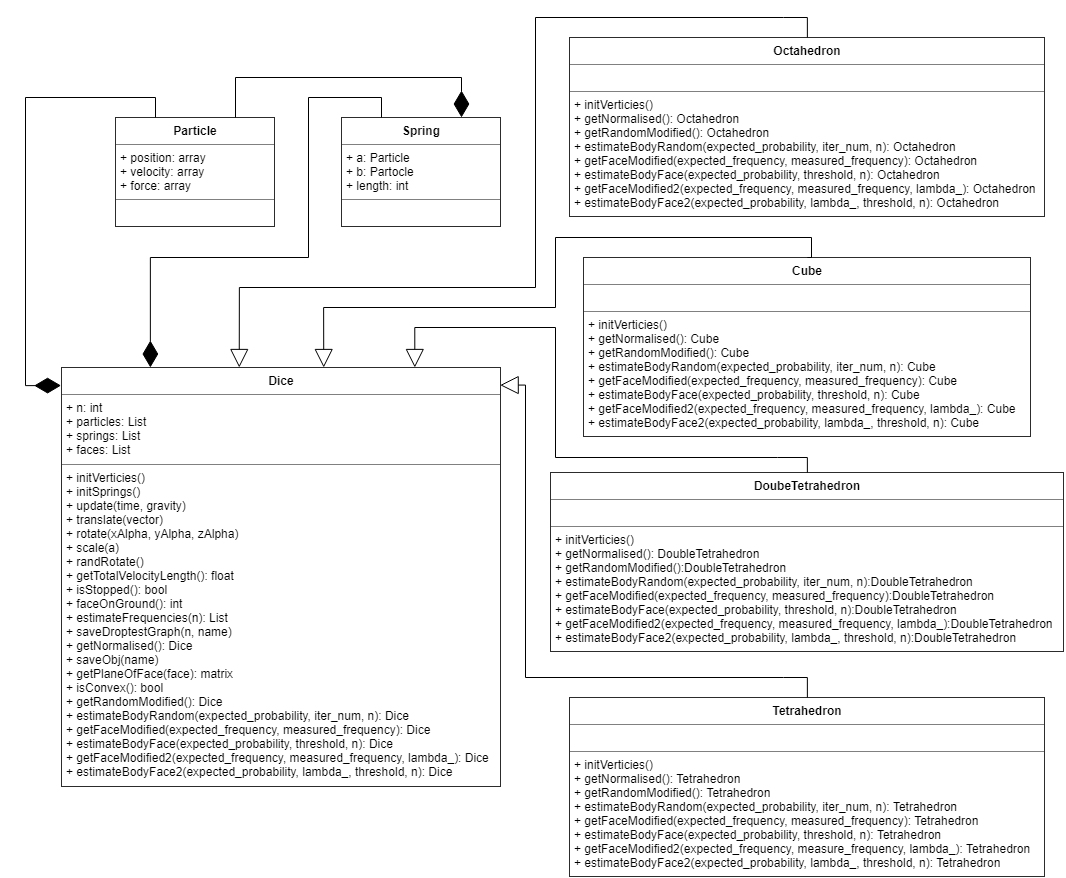
\includegraphics[width=\textwidth]{images/uml.png}
	\caption{Osztály diagram.}
	\label{fig:uml}
\end{figure}

\Aref{fig:uml} diagramon láthatóak a teszteléshez használt osztályok, és az azokhoz tartozó metódusok.
A \texttt{Particle} és a \texttt{Spring} osztály csak az adatok könnyebb, rendezett tárolásáért felelnek.

\SubSection{Pontok}

A pontok felelnek a test mozgásáért, a rá vonatkozó fizikai jellemzők itt találhatóak meg.
A szimulálás során a rá ható erőket, a mozgásvektorát, valamint a pozícióját tároljuk el.
Minden csúcs súlyát egységnyinek tekintjük, ezért nem foglalkozunk vele.

\begin{python}
class Particle:
    def __init__(self, a=[0, 0, 0]):
        self.position = np.array(a, dtype=float) 
        self.velocity = np.array([0, 0, 0], dtype=float)
        self.force = np.array([0, 0, 0], dtype=float)

    def __str__(self):
        return "({:.3f}, {:.3f}, {:.3f})".format(*self.position)
\end{python}

\SubSection{Rugók}

A rúgók felelnek a pontok helyén tartásáért.
A rugók miatt a testnek zselatinos jellege lesz (nyugalmi helyzetben is remegni fog).
Ezt a rugóállandóval lehet szabályozni.
Mivel homogén testekkel foglalkozunk, a rugóállandót konstansként kezeljük, ezért nem tároljuk el.

A test módosítása után a rugókat újra kell inicializálni, hogy a pontok közötti új távolságot próbálja meg folyamatosan tartani.
Ha ezt nem tennénk meg, a dobás szimulálása után a test visszaugrana a módosítás előtti állapotába.

\begin{python}
class Spring:
    def __init__(self, a, b):
        self.a = a
        self.b = b
        self.length = np.linalg.norm(self.b.position - self.a.position)
	
    def __str__(self):
        return f"{self.a}; {self.b}; {self.length}"
\end{python}

\SubSection{Konvexitásvizsgálat}

A dolgozat során csak a konvex testekkel fogunk foglalkozni, mivel könnyen belátható, hogy konkáv testek esetében lenne olyan oldallap, amelyre nem tud érkezni a dobás során a test.
Emiatt a módosítások után egy konvexitás vizsgálatot kell elvégeznünk a testen.
Ha a test konvex, akkor bármely oldallapjára nézve a pontok, amelyek nem csúcspontjai az oldalnak, ugyan abban az oldallap síkja által határolt félsíkban helyezkednek el.
Ehhez a vizsgálathoz fel kell írnunk minden oldallap síkjának az egyenletét, és a lapon kívüli pontokat vissza kell helyettesítenünk.
Ha minden pont ugyanabban a félsíkban található, akkor a behelyettesítéssel kapott értékek előjele meg fog egyezni.

Az oldallapok síkját úgy számoljuk, hogy az első három csúcspontjára ($P_1(x_1, y_1, z_1)$, $P_2(x_2, y_2, z_2)$ és $P_3(x_3, y_3, z_3)$) illesztjük a síkot az alábbi egyenletet használva:

\[
det(A)=0,\quad \text{ahol } A = 
\begin{bmatrix}
	x & y & z & 1 \\
	x_1 & y_1 & z_1 & 1 \\
	x_2 & y_2 & z_2 & 1 \\
	x_3 & y_3 & z_3 & 1
\end{bmatrix}.
\]

\begin{proof}
	A $P_1(x_1, y_1, z_1)$, $P_2(x_2, y_2, z_2)$ és $P_3(x_3, y_3, z_3)$ pont által meghatározott sík normálvektora:
	\[
	\begin{array}{c}
		\vec{n}=\overrightarrow{P_1 P_2}\times\overrightarrow{P_1 P_3}=(x_2-x_1, y_2-y_1, z_2-z_1)\times(x_3-x_1, y_3-y_1, z_3-z_1)=\\
		=
		\begin{vmatrix}
			\vec{i} & \vec{j} & \vec{k} \\
			x_2-x_1 & y_2-y_1 & z_2-z_1 \\
			x_3-x_1 & y_3-y_1 & z_3-z_1
		\end{vmatrix}=\\
		= ((y_2-y_1)(z_3-z_1)-(z_2-z_1)(y_3-y_1))\vec{i}+\\
		+ ((z_2-z_1)(x_3-x_1)-(x_2-x_1)(z_3-z_1))\vec{j}+\\
		+ ((x_2-x_1)(y_3-y_1)-(y_2-y_1)(x_3-x_1))\vec{k}
	\end{array}.
	\]
	A normálvektor és a $P1$ által felírt sík egyenlete:
	\[
	\begin{array}{c}
		A(x-x_1)+B(y-y_1)+C(z-z_1)=\\
		=((y_2-y_1)(z_3-z_1)-(z_2-z_1)(y_3-y_1))(x-x_1)+\\
		+((z_2-z_1)(x_3-x_1)-(x_2-x_1)(z_3-z_1))(y-y_1)+\\
		+((x_2-x_1)(y_3-y_1)-(y_2-y_1)(x_3-x_1))(z-z_1)=\\
		=(y_2 z_3 - y_1 z_3 - y_2 z_1 + y_1 z_1 - y_3 z_2 + y_3 z_1 + y_1 z_2 - y_1 z_1)(x-x_1)+\\
		+(x_3 z_2 - x_3 z_1 - x_1 z_2 + x_1 z_1 - x_2 z_3 + x_1 z_3 + x_2 z_1 - x_1 z_1)(y-y_1)+\\
		+(x_2 y_3 - x_1 y_3 - x_2 y_1 + x_1 y_1 - x_3 y_2 + x_3 y_1 + x_1 y_2 - x_1 y_1)(z-z_1)=\\
		=(y_2 z_3 - y_1 z_3 - y_2 z_1 - y_3 z_2 + y_3 z_1 + y_1 z_2)(x-x_1)+\\
		+(x_3 z_2 - x_3 z_1 - x_1 z_2 - x_2 z_3 + x_1 z_3 + x_2 z_1)(y-y_1)+\\
		+(x_2 y_3 - x_1 y_3 - x_2 y_1 - x_3 y_2 + x_3 y_1 + x_1 y_2)(z-z_1)=\\
		=(y_2 z_3 - y_1 z_3 - y_2 z_1 - y_3 z_2 + y_3 z_1 + y_1 z_2)x+\\
		+(x_3 z_2 - x_3 z_1 - x_1 z_2 - x_2 z_3 + x_1 z_3 + x_2 z_1)y+\\
		+(x_2 y_3 - x_1 y_3 - x_2 y_1 - x_3 y_2 + x_3 y_1 + x_1 y_2)z-\\
		- x_1 y_2 z_3 + x_1 y_1 z_3 + x_1 y_2 z_1 + x_1 y_3 z_2 - x_1 y_3 z_1 - x_1 y_1 z_2 -\\
		- x_3 y_1 z_2 + x_3 y_1 z_1 + x_1 y_1 z_2 + x_2 y_1 z_3 - x_1 y_1 z_3 - x_2 y_1 z_1 -\\
		- x_2 y_3 z_1 + x_1 y_3 z_1 + x_2 y_1 z_1 + x_3 y_2 z_1 - x_3 y_1 z_1 - x_1 y_2 z_1 =\\
		=(y_2 z_3 - y_1 z_3 - y_2 z_1 - y_3 z_2 + y_3 z_1 + y_1 z_2)x+\\
		+(x_3 z_2 - x_3 z_1 - x_1 z_2 - x_2 z_3 + x_1 z_3 + x_2 z_1)y+\\
		+(x_2 y_3 - x_1 y_3 - x_2 y_1 - x_3 y_2 + x_3 y_1 + x_1 y_2)z-\\
		- x_1 y_2 z_3 - x_2 y_3 z_1 - x_3 y_1 z_2 + x_3 y_2 z_1 + x_2 y_1 z_3  + x_1 y_3 z_2 = 0.
	\end{array}
	\]
	A $P_1(x_1, y_1, z_1)$, $P_2(x_2, y_2, z_2)$ és $P_3(x_3, y_3, z_3)$ pont által meghatározott sík egyenlete a feltételezésünk szerint:
	\[
	\begin{array}{c}
		A =
		\begin{vmatrix}
			x & y & z & 1 \\
			x_1 & y_1 & z_1 & 1 \\
			x_2 & y_2 & z_2 & 1 \\
			x_3 & y_3 & z_3 & 1
		\end{vmatrix}
		= x
		\begin{vmatrix}
			y_1 & z_1 & 1 \\
			y_2 & z_2 & 1 \\
			y_3 & z_3 & 1
		\end{vmatrix}
		- y
		\begin{vmatrix}
			x_1 & z_1 & 1 \\
			x_2 & z_2 & 1 \\
			x_3 & z_3 & 1
		\end{vmatrix}
		+ z
		\begin{vmatrix}
			x_1 & y_1 & 1 \\
			x_2 & y_2 & 1 \\
			x_3 & y_3 & 1
		\end{vmatrix}
		-
		\begin{vmatrix}
			x_1 & y_1 & z_1 \\
			x_2 & y_2 & z_2 \\
			x_3 & y_3 & z_3
		\end{vmatrix}
		=\\
		=(y_2 z_3 - y_1 z_3 - y_2 z_1 - y_3 z_2 + y_3 z_1 + y_1 z_2)x+\\
		+(x_3 z_2 - x_3 z_1 - x_1 z_2 - x_2 z_3 + x_1 z_3 + x_2 z_1)y+\\
		+(x_2 y_3 - x_1 y_3 - x_2 y_1 - x_3 y_2 + x_3 y_1 + x_1 y_2)z-\\
		- x_1 y_2 z_3 - x_2 y_3 z_1 - x_3 y_1 z_2 + x_3 y_2 z_1 + x_2 y_1 z_3  + x_1 y_3 z_2 = 0.
	\end{array}
	\]
	Mivel ugyan azt az egyenletet kaptuk, így beláthatjuk hogy a sík egyenlete megegyezik a $det(A)=0$ egyenlettel.
\end{proof}

Az egyenlet ilyen felírása azért előnyös a számunkra, mert a \texttt{numpy} könyvtár tartalmaz függvényt, amely mátrix determinánst számol.
Így csak a mátrix felírását kell megoldanunk, az első sorába behelyettesíteni a vizsgált pont koordinátáit majd a mátrix determinánsának előjele alapján eldönteni, hogy melyik félsíkon található a pont.
Nem szükséges tudnunk, hogy a pontok pontosan melyik félsíkban helyezkednek el, minket csak az érdekel, hogy oldalakra nézve minden vizsgált pontra a $det(A)$ érték előjele azonos legyen.
Ennek a megvalósításához az értékekhez rendelt \texttt{np.linalg.det(A) < 0} logikai értéket fogjuk eltárolni egy halmazban, majd a halmaz méretéről meg tudjuk állapítani, hogy összesen mennyi féltérben helyezkednek el a vizsgált pontok.
Ha minden oldal esetén a halmazban lévő elemek száma 1, akkor a test konvex.
Az alábbi metódusokat használjuk az oldallap síkjának meghatározására és a konvexitás vizsgálatára:

\begin{python}
def getPlaneOfFace(self, face):
    f = list(face)
    A = np.matrix([self.particles[f[0]].position,
                   self.particles[f[1]].position,
                   self.particles[f[2]].position])
    p = np.array([0, 0, 0])
    one = np.array([[1], [1], [1], [1]])
    A = np.vstack([p, A])
    A = np.append(A, one, axis=1)
    return A
    
def isConvex(self):
    for face in self.faces:
        A = self.getPlaneOfFace(face)
        sign = set()

        for i in range(self.n):
            if i not in face:
                A[0, :3] = self.particles[i].position
                sign.add(np.linalg.det(A) < 0)

        if len(sign) != 1:
            return False

    return True
\end{python}

\SubSection{Exportálás fájlba}

A programunk nem rendelkezik háromdimenziós megjelenítővel, ezért a testek megjelenítését külső programmal kell megtennünk, amihez a testeket WaveFront OBJ \cite{wavefrontOBJ} formátumú fájlba mentjük ki.
Azért erre esett a választás, mert ezeket a fájlokat a legtöbb 3D szerkesztő meg tudja nyitni, valamint az adattárolása megegyezik az általunk használt tárolási móddal.
Az exportálás az alábbi metódus formájában valósult meg.

\newpage

\begin{python}
def saveObj(self, name):
    filepath = f"objects/{name}.obj"

    with open(filepath, 'w') as f:
        f.write("# OBJ file\n")
        for particle in self.particles:
            f.write("v {} {} {}\n".format(*particle.position))
        for face in self.faces:
            f.write("f")
            for p in face:
                f.write(f" {p + 1}")
            f.write("\n")

    print(f"Obj file saved to '{filepath}'.")
\end{python}

\Section{Dobások}

A kockadobások szimulálását úgy végezzük, hogy a testet egy adott magasságig felemeljük, majd onnan ejtjük le a $z=0$ síkra.
A fizikai számításokat a \texttt{Dice.update} metódus végzi el az alábbi lépéssorozatot követve:
\begin{enumerate}
	\item A csúcspontokra ható erőt beállítja a gravitációs erőre.
	\item Az erőhöz hozzáadja a csúcspont mozgásvektorát.
	\item Kiszámítja a rugóerőket, és rendre hozzáadja/kivonja az erőkből.
	\item Ha egy pont a $z=0$ síkon, vagy alatta helyezkedik el, akkor kezeli a visszapattanást.
	\item Az erőkből kiszámítja a pontok új mozgásvektorait.
	\item A csúcsokat mozgatja a mozgásvektoruknak megfelelően .
\end{enumerate}
A szimulációnak nem célja, hogy fizikálisan pontos legyen, mivel a testeknek csak az alakja érdekel minket.
Emiatt az iterációk között eltelt időt egységnyinek tekintjük, és hozzá állítottunk be egy lefelé mutató vektort konstans gravitációs erőnek.

\SubSection{Véletlenszerű forgatás}
\label{subs:randompoint}

Azért, hogy a test véletlenszerűen érkezzen az egyik oldalára, a leejtés szimulálása előtt el kell forgatnunk úgy, hogy minden lehetséges pozíció ugyan akkora valószínűséggel forduljon elő.
Ehhez viszont nem elegendő három $0^\circ \leq \alpha_x,\alpha_y,\alpha_z <360^\circ$ szöget választanunk véletlenszerűen és azokkal elforgatnunk az $x$, $y$ és $z$ tengely körül.
\begin{proof}
Amennyiben a szimulációnk hiteles, szabályos kocka esetén a $0^\circ \leq \alpha_x,\alpha_y,$ $\alpha_z <360^\circ$ szögekkel való forgatás helyettesíthető azzal a módszerrel, hogy csak $0^\circ$, $90^\circ$, $180^\circ$ vagy $270^\circ$-kal forgatjuk a tengelyek mentén. Így a kockát összesen $4\cdot 4\cdot 4 = 64$ módon tudjuk forgatni. Mivel a kapott érték nem osztható hattal, így beláthatjuk, hogy a forgatás után történő dobás eloszlása nem egyenletes lesz. 
\end{proof}

\noindent Az egyenletes forgatáshoz az alábbi algoritmust használjuk.
\begin{enumerate}
	\item Kiválasztjuk az egyik csúcspontot pivotnak.
	\item Választunk egy $R$ pontot az origó-pivot sugarú gömbfelületén.
	\item Úgy forgatjuk a testet, hogy a pivot pont az $R$ pontba essen.
	\item A testet elforgatjuk az origó és $R$  pontokon áthaladó egyenes körül egy $0^\circ \leq \alpha < 360^\circ$ szögel.
\end{enumerate}
\begin{remark}
Feltételezzük hogy a test középpontja az origóban van.
\end{remark}
Az implementálásban annyi különbség van, hogy nem a 4. lépésben leírt egyenes körül forgatjuk a testet.
Mielőtt a pivot csúcsot a választott pontba forgatnánk, úgy forgatjuk a testet, hogy a pivot illeszkedjen az $x$ tengelyre.
Ekkor végezzük el a 4. lépésben leírt forgatást, majd ezután forgatjuk a választott csúcsot az $R$ ponthoz.
Ez a változtatás nem befolyásolja a kapott forgatást.

Az $R$ pont egyenletes eloszlással történő választásához a gömbfelületen az $x_r, y_r$ és $z_r$ értékeket a sztenderd normális eloszlás szerint választjuk, majd normalizáljuk, és felszorozzuk a gömb sugarával.

A Box-Muller transzformáció \cite{boxmuller} segítségével két egyenletes eloszlású változó segítségével generálhatunk két normális eloszlású változót. Ebből beláthatjuk az egyenletes és normális eloszlás közötti összefüggés.

\SubSection{Leállási feltételek}

A szimuláció során leejtett testünk sosem fog teljesen megállni a rugók miatt, mindig kicsit vibrálni fog, emiatt a szimulációt addig futtatjuk, amíg a csúcspontok mozgásvektorainak az összhosszúsága egy küszöbérték alá nem esik.
Hogy kizárjuk annak a lehetőségét, hogy a test a fent említett kritériumnak megfelel, de egyik oldalára sem érkezett, ezért meg kell számolni hogy hány csúcs található a $z=0$ sík közelében. (A folyamatos pattogás és rezgés miatt itt is egy küszöbértékhez kell viszonyítanunk.)

\begin{figure}[h!]
	\centering
	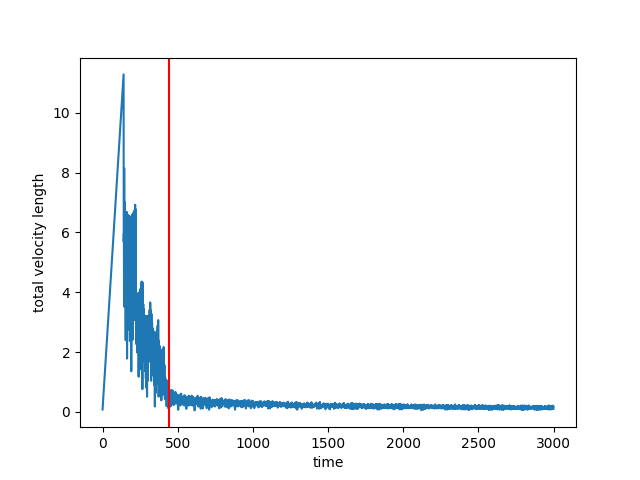
\includegraphics[scale=0.7]{images/cube_normal_3000.png}
	\caption{Szabályos, forgatás nélküli kocka ejtése közben mért mozgásvektorok összhosszúsága az idő függvényében.}
	\label{fig:cn3000}
\end{figure}
\begin{figure}[h!]
	\centering
	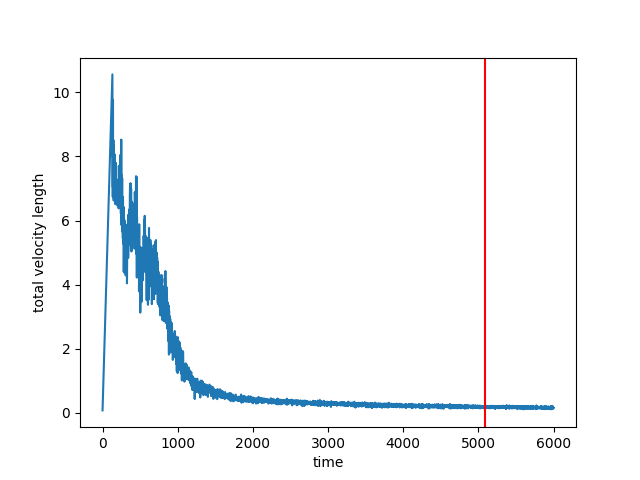
\includegraphics[scale=0.7]{images/cube_rotated_6000.png}
	\caption{Szabályos, forgatott kocka ejtése közben mért mozgásvektorok összhosszúsága az idő függvényében.}
	\label{fig:cr6000}
\end{figure}
A mért értékek alapján a mozgásvektorok összhoszzúságához tartozó küszöbérték $0.13$, a $z$ értékekre pedig $0.001$.
A \ref{fig:cn3000} és a \ref{fig:cr6000} ábrán a vörös függőleges vonal jelzi azt a pontot, amikor a program a már említett paraméterekkel megálltnak titulálta a kockát.
Látható, hogy az ideális pozícióból ejtett test sokkal hamarabb megáll, mint a forgatott.
Az elforgatott kocka nem sokkal az 5000. iteráció után megáll a talajon.
Nem szabályos test esetén arra számítunk, hogy kevesebb mint 10000 iteráció alatt meg fog állni a test.
Ha ez nem történne meg az első 10000 iterációban (egy élén vagy csúcsán pattog a végtelenségig), akkor a dobást érvénytelennek tekintjük.

\newpage

\SubSection{Kiértékelés}

A módosított testeknél gyakran a dobás értéke nem rendelhető egy "felül lévő" laphoz, mint a kocka esetében, ezért célszerű a dobott értékeket a $z=0$ síkon lévő laphoz rendelni.
Hasonlóan a leállás vizsgálatához, eltároljuk egy halmazban a talajon található pontok indexeit, majd megkeressük hogy melyik oldallap a részhalmaza.

A következő metódus adja vissza a talajon lévő oldallapnak az indexét.
Látható, hogy különböző negatív értéket ad vissza, ha a test nem állt meg, nem tudunk egy lapot sem észlelni, vagy ha egyszerre több lapot is hozzá tudunk rendelni a dobáshoz.
A különböző értékekre a tervezési fázisban volt szükség, hogy tudjuk hogy miért nem kaptunk egyes esetekben eredményt.
A kész programban ilyen hibák ritkán fordulnak elő, az előfordulásuk esetén a dobást megismételjük.
Ez a megközelítés azért helytálló, mert ha tartósan rossz eredményeket kapunk, az meglátszódik a mért gyakoriságokon, és a test módosító algoritmusok ezeket ki tudják javítani.

\begin{python}
def faceOnGround(self):
    if not self.isStopped():
        print("not stopped")
        return -1

    onGround = set()
    for i in range(self.n):
        if self.particles[i].position[2] < ZMIN:
            onGround.add(i)

    face = []
    for i in range(len(self.faces)):
        if self.faces[i].issubset(onGround):
            face.append(i)

    if len(face) == 0:
        print("no face detected")
        return -2
    elif len(face) == 1:
        return face[0]
    else:
        print("multiple faces detected")
        return -3
\end{python}

\newpage

A dobássorozatokkal kapott gyakoriságokat egy tömbben tároljuk el, ahol a gyakoriságok indexei megegyeznek a hozzájuk tartozó oldallap indexével.

\begin{python}
def estimateFrequencies(self, n):
    stat = [0] * len(self.faces)

    height = 100
    dropHeight = np.array([0, 0, height], dtype=float)

    while sum(stat) < n:
        tmp = deepcopy(self)

        c = tmp.getCenter()
        tmp.translate(-1 * c)
        tmp.randRotate()
        tmp.translate(c)
        tmp.translate(dropHeight)

        i = 0
        while (not tmp.isStopped()) and i < MAXITER:
            tmp.update(TIME, GRAVITY)
            i += 1

        index = tmp.faceOnGround()
        if index >= 0:
            stat[index] += 1

    return stat
\end{python}

Az így kapott tömb elemein fogunk statisztikai vizsgálatokat végezni, hogy tudjuk a testet az elvárt eloszláshoz módosítani.
Az egyes algoritmusok részletezése a következő fejezetben található.